\section{Technology Assessment}
\label{sec:technology}

Elm was created by Evan Czaplicki in 2012 and was designed to simplify front-end development. By addressing common issues such as runtime errors and large, complex codebases, Czaplicki envisioned a tool that prioritised developer productivity and application reliability. This was achieved by combining the principles of functional programming with a focus on usability. Elm eliminates entire classes of runtime errors through its type-safe design while producing highly optimised and minimalistic deployment bundles. Its philosophy emphasises simplicity, predictability, and a delightful developer experience.

\begin{figure}[thb]
	\centering
	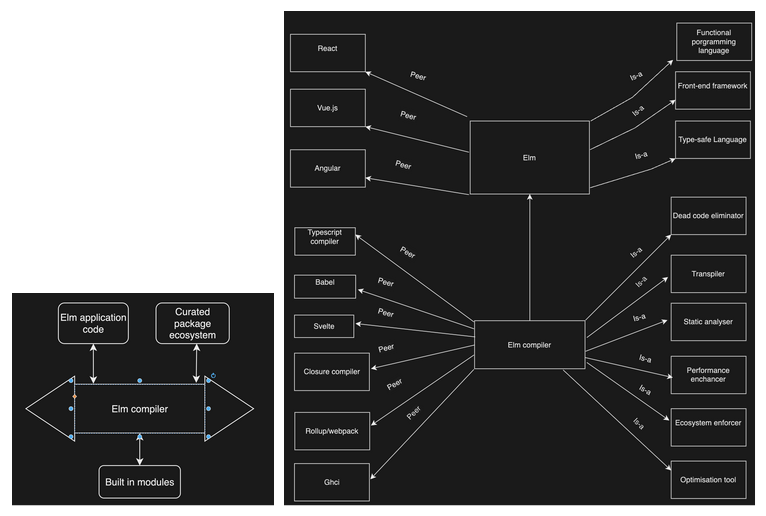
\includegraphics[scale=0.5]{figs/diagram.png}
	\caption{Figure.}
	\label{fig:diagram}
\end{figure}

\subsection{Elm's Ecosystem}
Figure 3 illustrates the key elements of Elm’s ecosystem. At its center is the \textbf{Elm Compiler}, which links application code, built-in modules, and a curated package ecosystem. This integration allows Elm to streamline and optimise the code it generates. Unlike frameworks like React or Angular, there is no dependence on separate build tools, as Elm’s compiler performs all optimisations directly, including removing unnecessary dependencies to reduce deployment size.

Figure 4 highlights Elm's relationships within the broader genealogy. Elm \textit{"is-a"} functional programming language and front-end framework. It emphasises immutability and type safety, setting it apart from traditional frameworks. Elm’s compiler also serves as a peer to tools like the TypeScript Compiler, Babel, and Svelte. While these tools aim to optimise and transform code, Elm’s compiler enforces consistency across its ecosystem, helping produce smaller and more predictable deployment bundles.

\section{Problem Domain Habitat}
Elm addresses significant challenges in front-end development. Managing application complexity, ensuring runtime reliability, and producing efficient deployment bundles are all areas Elm seeks to improve. Its approach is particularly suited to environments where application reliability and asset size are critical considerations. Unlike frameworks like React and Angular, which rely heavily on runtime libraries, Elm's architecture eliminates runtime exceptions through compile-time guarantees.

\begin{figure}[thb]
	\centering
	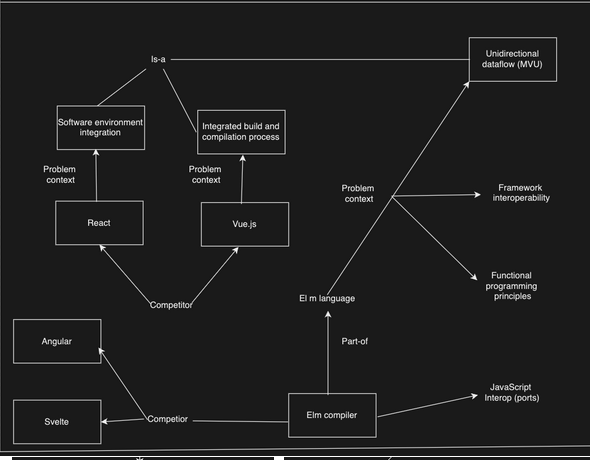
\includegraphics[scale=0.5]{figs/diagram2.png}
	\caption{Figure.}
	\label{fig:diagram2}
\end{figure}

Figure 5 depicts Elm competing with React, Vue.js, Svelte, and Angular in the domain of front-end frameworks. These tools address common issues such as state management, component reuse, and rendering efficiency. Elm distinguishes itself through its \textbf{Model-View-Update (MVU)} architecture, enforcing unidirectional data flow. This simplifies application logic and enables the compiler to produce highly optimised and minimalistic outputs.

Additionally, Elm supports JavaScript interoperability via \textbf{ports}, allowing integration with existing JavaScript codebases. This makes it feasible for developers to adopt Elm incrementally within larger applications. However, Elm’s curated package ecosystem and strict typing model put emphasis on stability over flexibility, distinguishing it from competitors that prioritise rapid prototyping or experimental features.

Elm excels in scenarios where predictable performance, maintainability, and minimal runtime overhead are critical, such as performance-critical web applications or bandwidth-constrained environments. Conversely, Elm’s limited ecosystem flexibility may be less suitable for projects needing extensive third-party library support.

\section{Experiment Design Phase}

\subsection{Comparative Feature Analysis}
The comparative feature analysis examines the features influencing deployment asset size in Elm, React, Vue, and Svelte. The reference model focuses on features that impact deployment size, including:

\begin{itemize}
    \item \textbf{Code Optimization:} Elm's compiler removes unused code and generates efficient JavaScript. React, Vue, and Svelte rely on external build tools like Webpack, which require proper configuration to avoid unused dependencies.
    \item \textbf{Dependency Management:} Elm uses a curated package system to reduce unnecessary libraries. React, Vue, and Svelte allow broader use of third-party dependencies, increasing the risk of bloated deployment assets.
    \item \textbf{Runtime Overhead:} Elm's functional programming model avoids runtime processes for dynamically updating the user interface, resulting in smaller runtime sizes. Svelte employs a similar compile-time approach. React and Vue use runtime processes to track and update changes, increasing final application size.
    \item \textbf{State Management:} Elm's MVU architecture simplifies state management at compile time, reducing runtime overhead. React uses unidirectional data flow with hooks and stateful components, Vue offers reactive data binding, and Svelte compiles reactive assignments into efficient JavaScript.
    \item \textbf{JavaScript Integration:} Elm uses \textit{ports} for JavaScript integration, which can slightly increase bundle size in hybrid apps. React, Vue, and Svelte natively integrate with JavaScript, but bundle size increases with multiple libraries.
\end{itemize}

\subsection{Feature Deltas}
Feature deltas highlight how Elm integrates its language, architecture, and compiler to reduce redundant dependencies and produce smaller bundles. React, Vue, and Svelte focus on runtime flexibility, often leading to larger deployment assets.

\subsection{Hypothesis Formulation}
From the analysis, the following hypothesis is formulated:
\begin{quote}
    \textit{"Applications written in Elm produce smaller deployment assets compared to applications written in popular frameworks like React, Vue, or Svelte for equivalent functionality."}
\end{quote}

The hypothesis is supported by:
\begin{enumerate}
    \item \textbf{Integrated Compiler:} Elm’s compiler optimises code at the source, reducing reliance on external tools.
    \item \textbf{Curated Ecosystem:} Elm's package system includes only essential libraries, avoiding unnecessary dependencies.
    \item \textbf{Functional Design:} Elm's declarative style and MVU model reduce redundant code and ensure smaller deployment assets.
    \item \textbf{Feature Deltas:} Elm prioritises efficiency compared to the runtime-heavy approaches of React, Vue, and Svelte.
\end{enumerate}

\subsection{Experiment Design}
The experiment involves two main approaches: \textbf{synthetic benchmarks} and a \textbf{demonstrator study}.
\begin{itemize}
    \item Synthetic benchmarks involve creating naive implementations of simple applications (e.g., "Hello World," counter, GET request) in Elm, React, Vue, and Svelte. These are used to compare how deployment assets scale with increasing complexity.
    \item The demonstrator study assesses Elm's functionality through the development of a poll application, evaluating lessons learned, compatibility with JavaScript applications, and the consequences of Elm’s unique features.
\end{itemize}

\section{Experiment Evaluation Phase}


\subsection{Synthetic Benchmarks}
The benchmarks revealed that Elm's asset size grows more rapidly compared to other frameworks. While Elm eliminates unused dependencies, its need to explicitly import common features (e.g., HTML elements, HTTP requests) increases the number of dependencies in each application, resulting in larger asset sizes. Conversely, React, Vue, and Svelte include these features in their core libraries, maintaining relatively constant sizes.

\begin{figure}[thb]
	\centering
	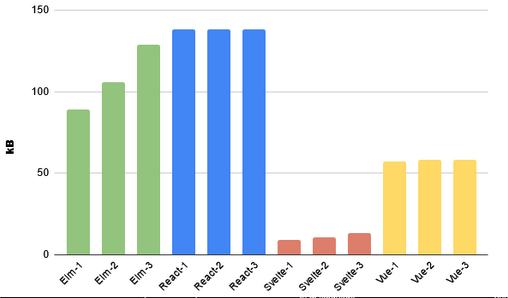
\includegraphics[scale=0.5]{figs/diagram3.png}
	\caption{Figure.}
	\label{fig:diagram3}
\end{figure}

\subsection{Demonstrator Study}
\textbf{General Observations:} Elm's steep learning curve posed challenges, especially for developers new to its architecture. While feature development was slower, its functional programming paradigm ensured reliability.

\textbf{Results:} Elm’s deployed site had an average page size of \textasciitilde 140kB. Consolidating pages into a single SPA could potentially save up to 60\% of the asset size by sharing common imports. The demonstrator study highlighted the importance of Elm's port and subscription system for interoperability with JavaScript applications, such as local storage access.

While the study discredits Elm's size advantage, it reinforces Elm’s strengths in reliability and maintainability through its type-safe, compiler-driven architecture.